\documentclass[14pt,a4paper]{report}  %紙張設定
\usepackage{xeCJK}%中文字體模組
%\setCJKmainfont{標楷體} %設定中文字體
\setCJKmainfont{MoeStandardKai.ttf}
%\newfontfamily\sectionef{Times New Roman}%設定英文字體
\newfontfamily\sectionef{Nimbus Roman}
\usepackage{enumerate}
\usepackage{amsmath,amssymb}%數學公式、符號
\usepackage{amsfonts} %數學簍空的英文字
\usepackage{graphicx, subfigure}%圖形
\usepackage{fontawesome5} %引用icon
\usepackage{type1cm} %調整字體絕對大小
\usepackage{textpos} %設定文字絕對位置
\usepackage[top=2.5truecm,bottom=2.5truecm,
left=3truecm,right=2.5truecm]{geometry}
\usepackage{titlesec} %目錄標題設定模組
\usepackage{titletoc} %目錄內容設定模組
\usepackage{textcomp} %表格設定模組
\usepackage{multirow} %合併行
%\usepackage{multicol} %合併欄
\usepackage{CJK} %中文模組
\usepackage{CJKnumb} %中文數字模組
\usepackage{wallpaper} %浮水印
\usepackage{listings} %引用程式碼
\usepackage{hyperref} %引用url連結
\usepackage{setspace}
\usepackage{lscape}%設定橫式
\lstset{language=Python, %設定語言
		basicstyle=\fontsize{10pt}{2pt}\selectfont, %設定程式內文字體大小
		frame=lines,	%設定程式框架為線
}
%\usepackage{subcaption}%副圖標
\graphicspath{{./../images/}} %圖片預設讀取路徑
\usepackage{indentfirst} %設定開頭縮排模組
\renewcommand{\figurename}{\Large 圖.} %更改圖片標題名稱
\renewcommand{\tablename}{\Large 表.}
\renewcommand{\lstlistingname}{\Large 程式.} %設定程式標示名稱
\hoffset=-5mm %調整左右邊界
\voffset=-8mm %調整上下邊界
\setlength{\parindent}{3em}%設定首行行距縮排
\usepackage{appendix} %附錄
\usepackage{diagbox}%引用表格
\usepackage{multirow}%表格置中
%\usepackage{number line}
%=------------------更改標題內容----------------------=%
\titleformat{\chapter}[hang]{\center\sectionef\fontsize{20pt}{1pt}\bfseries}{\LARGE 第\CJKnumber{\thechapter}章}{1em}{}[]
\titleformat{\section}[hang]{\sectionef\fontsize{18pt}{2.5pt}\bfseries}{{\thesection}}{0.5em}{}[]
\titleformat{\subsection}[hang]{\sectionef\fontsize{18pt}{2.5pt}\bfseries}{{\thesubsection}}{1em}{}[]
%=------------------更改目錄內容-----------------------=%
\titlecontents{chapter}[11mm]{}{\sectionef\fontsize{18pt}{2.5pt}\bfseries\makebox[3.5em][l]
{第\CJKnumber{\thecontentslabel}章}}{}{\titlerule*[0.7pc]{.}\contentspage}
\titlecontents{section}[18mm]{}{\sectionef\LARGE\makebox[1.5em][l]
{\thecontentslabel}}{}{\titlerule*[0.7pc]{.}\contentspage}
\titlecontents{subsection}[4em]{}{\sectionef\Large\makebox[2.5em][l]{{\thecontentslabel}}}{}{\titlerule*[0.7pc]{.}\contentspage}
%=----------------------章節的間距----------------------=%
\titlespacing*{\chapter} {0pt}{0pt}{18pt}
\titlespacing*{\section} {0pt}{12pt}{6pt}
\titlespacing*{\subsection} {0pt}{6pt}{6pt}
%=----------------------標題-------------------------=%             
\begin{document} %文件
\sectionef %設定英文字體啟用
\vspace{12em}
\begin{titlepage}%開頭
\begin{center}   %標題  
\makebox[1.5\width][s] %[s] 代表 Stretch the interword space in text across the entire width
{\fontsize{24pt}{2.5pt}國立虎尾科技大學}\\[18pt]
\makebox[1.5\width][s]
{\fontsize{24pt}{2.5pt}機械設計工程系}\\[18pt]
\sectionef\fontsize{24pt}{1em}\selectfont\textbf
{
\vspace{0.5em}
cd2023 2b-pj3bg3分組報告}\\[18pt]
%設定文字盒子 [方框寬度的1.5倍寬][對其方式為文字平均分分布於方框中]\\距離下方18pt
\vspace{1em} %下移
\fontsize{30pt}{1pt}\selectfont\textbf{網際足球場景設計}\\
\vspace{1em}
\sectionef\fontsize{30pt}{1em}\selectfont\textbf
{
\vspace{0.5em}
Web-based Football Scene Design}
 \vspace{2em}
%=---------------------參與人員-----------------------=%             
\end{center}
\begin{flushleft}
\begin{LARGE}

\hspace{32mm}\makebox[5cm][s]
{指導教授:\quad 嚴\quad 家\quad 銘\quad 老\quad 師}\\[6pt]
\hspace{32mm}\makebox[5cm][s]
{班\qquad 級:\quad 四\quad 設\quad 二\quad 乙}\\[6pt]
\hspace{32mm}\makebox[5cm][s]
{學\qquad 生:\quad 陳\quad 冠\quad 珉\quad(41023220)}
\\[6pt]
\hspace{32mm}\makebox[5cm][s]
{\hspace{36.5mm}陳\quad 建\quad 霖\quad(41023226)}\\[6pt]
\hspace{32mm}\makebox[5cm][s]
{\hspace{36.5mm}彭\quad 聖\quad 宗\quad(41023230)}\\[6pt]
\hspace{32mm}\makebox[5cm][s]
{\hspace{36.5mm}湛\quad 有\quad 杰\quad(41023231)}\\[6pt]
\hspace{32mm}\makebox[5cm][s]
{\hspace{36.5mm}雲\quad 敬\quad 家\quad(41023232)}\\[6pt]
\hspace{32mm}\makebox[5cm][s]
{\hspace{36.5mm}黃\quad 文\quad 彥\quad(41023233)}\\[6pt]
\hspace{32mm}\makebox[5cm][s]
{\hspace{36.5mm}蔡\quad 叡\quad 得\quad(41023250)}\\[6pt]
\hspace{32mm}\makebox[5cm][s]
{\hspace{36.5mm}謝\quad 宗\quad 銘\quad(41023253)}\\[6pt]
\hspace{32mm}\makebox[5cm][s]

%設定文字盒子[寬度為5cm][對其方式為文字平均分分布於方框中]空白距離{36.5mm}\空白1em
\end{LARGE}
\end{flushleft}
\vspace{6em}
\fontsize{18pt}{2pt}\selectfont\centerline{\makebox[\width][s]
{中華民國\hspace{3em} 
112 \quad 年\quad 6\quad 月}}
\end{titlepage}
\newpage

%=------------------------摘要-----------------------=%
\renewcommand{\baselinestretch}{1.5} %設定行距
\pagenumbering{roman} %設定頁數為羅馬數字
\clearpage  %設定頁數開始編譯
\sectionef
\addcontentsline{toc}{chapter}{摘~~~要} %將摘要加入目錄
\begin{center}
\LARGE\textbf{摘~~要}\\
\end{center}
\begin{flushleft}
\fontsize{14pt}{20pt}\sectionef\hspace{12pt}\quad 本專案旨在進行協同設計,以改良並優化雙輪車或多輪車,並應用於機器人足球比賽中。該專案分為三個階段,其中專案三是對專案二的延續。團隊組成包含8名成員,並使用CAD軟體進行場景和多輪車零組件的設計。透過採用ZmqRemoteAPI Python編程,開發控制程式以支持操控多輪車在足球場景中進行比賽。\\[12pt]

\fontsize{14pt}{20pt}\sectionef\hspace{12pt}\quad 專案三的目標是改進雙輪車或多輪車的行進和對戰效能。為了達到這一目標,團隊需要優化運動控制,使其能夠靈活且精確地操控。同時,引入協同運動策略,使多輪車能夠協調工作,並在比賽中進行合作攻守。為了提高對環境和球場的感知能力,團隊需要適當地選擇和應用感應器和感知系統。\\[12pt]

\fontsize{14pt}{20pt}\sectionef\hspace{12pt}\quad 在控制系統優化的過程中,團隊將進行模擬和測試,並根據實際結果和需求不斷進行改進和優化。最終,團隊將提供相關檔案的下載連結,並製作線上簡報和分組報告,以展示協同設計流程和成果。\\[12pt]

\fontsize{14pt}{20pt}\sectionef\hspace{12pt}\quad 透過這個協同設計的機器人踢足球專案,團隊將獲得實踐協同工作和創新的機會,同時提升雙輪車或多輪車在足球比賽中的性能和效能。這將為未來的機器人技術和運動應用帶來新的發展和應用前景。\\[12pt]
\end{flushleft}
\newpage
%=--------------------Abstract----------------------=%
\newpage
\renewcommand{\baselinestretch}{1.5} %設定行距

%=------------------------誌謝----------------------=%
\begin{center}	
\addcontentsline{toc}{chapter}{誌~~~謝}
\LARGE\textbf{誌~~謝}\\
\end{center}
\begin{center}
\begin{flushleft}
\fontsize{14pt}{20pt}\sectionef\hspace{12pt}\quad 在此鄭重感謝製作以及協助本分組報告完成的所有人員,首先向嚴家銘老師致謝,他解決我們的各種提問,甚至從來沒有不耐煩,總是貼心為我們找出最佳解答,接著是由OpenAI創造的ChatGPT,在我們需要創作的時候,他總能提供我們源源不斷的創意,最後是由本分組成員同心協力才得以完成本報告,特此感謝

\end{flushleft}
\newpage
%=------------------------目錄----------------------=%
\renewcommand{\contentsname}{\centerline{\fontsize{18pt}{\baselineskip}\selectfont\textbf{目\quad 錄}}}
\tableofcontents  %目錄產生
\newpage

\end{center}
%=-------------------------內容----------------------=%

\chapter{更新團隊網站步驟}
\section{詳細步驟說明}


 1.先開起個人USB中的倉儲ipv6\\

2.在至個人github中的fork倉儲更新成最新版\\

3.輸入git pull若失敗則有可能PUTTY跑掉重設定即可\\

4.進行編輯\\

5.acp\\

6.在至個人fork倉儲Open pull request\\

7.若無法pull request 那就至個人fork在合併最新版本並除錯即可\\

8.一路同意推送合併到底\\

9.回到整組倉儲確認上傳己完成\\




\chapter{pj3}



專案三: 接續專案二, 各組需對雙輪車進行設計改良,  以提升行進與對戰效能, 各組需採 CAD 進行場景與多輪車零組件設計後, 轉入足球場景中以鍵盤 arrow keys 與 wzas 等按鍵進行控制, 對陣雙方每組將有四名輪車球員, 且每兩人在同一台電腦上操作, 完成後各組需在分組網站中提供所有相關檔案下載連結, 且提供線上分組簡報與分組 pdf 報告連結.\\

球賽計分系統必須採 .ttm 格式建立 (0~99), 使能通用於各類場景計數之用, 並可擴增至三位數計分.\\

除了採用 LED 顯示計分外, 請另外以建立以機械轉盤傳動計分系統 (mechanical counter), 且採 .ttm 格式建立.\\

協同產品設計規格:\\

足球規格 (ball): 白色, 直徑 0.1m, 重量 0.5kg\\

足球場地 (field): 長 4m x 寬 2.5m\\

球門規格 (goal[0] and goal[1]: 長 0.6m, 高 0.3m, 寬 0.1m\\

球員尺寸範圍(player[0]-player[7]: 長寬高各 0.2m, 重量 5kg\\


應交付內容:\\

專案三場景與多輪車零組件設計 (可使用各種 CAD 系統建立, 但必須提供完整的檔案下載連結)\\

專案三控制程式 (以 zmqRemoteAPI Python 製作)\\

專案三開會紀錄與逐字稿 (可利用 jit.si 或 OBS 或其他線上開會系統)\\

專案三各組員任務分配與執行過程影片 (可置於 Youtube 或 Onedrive)\\

專案三網站包括所有協同設計流程所衍生的檔案下載連結, 各檔案必須設法壓縮在 30 MB 內並置於網站downloads 目錄中.\\

專案三線上簡報檔案\\

專案三分組報告 pdf 檔案\\

直接利用 zmqRemoteAPI Python 程式建立場景物件:\\
\begin{lstlisting}[language=Python, frame=single, numbers=left, captionpos=b, basicstyle=\ttfamily\small, showstringspaces=false, breaklines=true, tabsize=4, xleftmargin=15pt]
# zmqRemoteApi_IPv6 為將 zmq 通訊協定修改為 IPv4 與 IPv6 相容
from zmqRemoteApi_IPv6 import RemoteAPIClient
import time
import math
import keyboard
 
# 利用 zmqRemoteAPI 以 23000 對場景伺服器進行連線
client = RemoteAPIClient('localhost', 23000)
# 以 getObject 方法取得場景物件
sim = client.getObject('sim')
box = sim.getObject('/box')
 
# 啟動模擬
sim.startSimulation()
# 建立尺寸數列, 分別定義 x, y, z 方向尺寸
x = 0.2
y = 0.2
z = 0.1
size = [x, y, z]
 
# 利用 size 數列, 建立圓柱物件, 2 代表 cylinder
# 8 表示 respondable, 1 為 質量
digit1_handle = sim.createPureShape(2, 8, size, 1, None)
# 將圓柱物件命名為 digit1, 若用於機械計分可做為個位數轉盤
# 之後可再導入帶有數字組立的外型零件
sim.setObjectAlias(digit1_handle, 'digit1')
# 轉角單位為徑度
sim.setObjectOrientation(digit1_handle, -1, [0, math.pi/2, 0])
# 起始物件中心位於 [0, 0, 0], 為了位於地板, 往 z 提升一個半徑高度
sim.setObjectPosition(digit1_handle, -1, [0, 0, x/2])
 
# 建立 revolute joint 命名為 joint, 且將 joint mode 設為 dynamic, control mode 設為 velocity
joint1_handle = sim.createJoint(sim.joint_revolute_subtype, sim.jointmode_dynamic, 0, None)
sim.setObjectInt32Param(joint1_handle, sim.jointintparam_dynctrlmode, sim.jointdynctrl_velocity)
sim.setObjectAlias(joint1_handle, 'joint1')
 
# 取得 cylinder 的位置座標
digit1_pos = sim.getObjectPosition(digit1_handle, -1)
joint1_pos = [digit1_pos[0], digit1_pos[1], digit1_pos[2]]
 
# 將 joint1 至於 cylinder 中心
sim.setObjectPosition(joint1_handle, -1, joint1_pos)
# 取得 digit1_handle 的方位
digit1_ori = sim.getObjectOrientation(digit1_handle, -1)
# 將 joint1_handle 方位與 digit1 對齊
sim.setObjectOrientation(joint1_handle, -1, digit1_ori)
 
# 將 joint1 置於 box 上
sim.setObjectParent(joint1_handle, box, True)
# 將 cylinder 置於 joint1 上
sim.setObjectParent(digit1_handle, joint1_handle, True)
 
# 鎖定 joint1
sim.setJointForce(joint1_handle, float('inf'))
 
print("基本場景建立完成!")
 
# 設定主迴圈
while True:
    # 設定 joint1 目標速度
    sim.setJointTargetVelocity(joint1_handle, 10)
    # 讓 coppeliasim 有時間按照設定讓 joint1 旋轉
    time.sleep(0.01) 
 
    if keyboard.is_pressed('q'):
        # 可以按下 q 鍵跳出重複執行迴圈
        break
 
# 終止模擬
#sim.stopSimulation()
\end{lstlisting}

\chapter{code}
\section{code\_car}
第一版程式,使用兩邊的速度差來控制方向,且可以在前後的同時控制方向\\
\begin{lstlisting}[language=Python, frame=single, numbers=left, captionpos=b, basicstyle=\ttfamily\small, showstringspaces=false, breaklines=true, tabsize=4, xleftmargin=15pt]
from zmqRemoteApi_IPv6 import RemoteAPIClient
import keyboard
 
client = RemoteAPIClient('localhost', 23000)
 
print('Program started')
sim = client.getObject('sim')
sim.startSimulation()
print('Simulation started')
 
def setWheelMotion(leftSpeed, rightSpeed):
    # Set target velocity for each wheel
    frontLeftWheel = sim.getObject('/frontLeftJoint')
    frontRightWheel = sim.getObject('/frontRightJoint')
    rearLeftWheel = sim.getObject('/rearLeftJoint')
    rearRightWheel = sim.getObject('/rearRightJoint')
    sim.setJointTargetVelocity(frontLeftWheel, leftSpeed)
    sim.setJointTargetVelocity(frontRightWheel, rightSpeed)
    sim.setJointTargetVelocity(rearLeftWheel, leftSpeed)
    sim.setJointTargetVelocity(rearRightWheel, rightSpeed)
 
# Initialize motion variables
leftSpeed = 0
rightSpeed = 0
 
# Main loop
while True:
    # Check keyboard input
    if keyboard.is_pressed('w'):
        leftSpeed = -10  # Forward motion
        rightSpeed = -10  # Forward motion
    elif keyboard.is_pressed('s'):
        leftSpeed = 10  # Backward motion
        rightSpeed = 10  # Backward motion
    else:
        leftSpeed = 0
        rightSpeed = 0
 
    if keyboard.is_pressed('a'):
        leftSpeed += 5  # Left turn
        rightSpeed -= 5  # Left turn
    elif keyboard.is_pressed('d'):
        leftSpeed -= 5  # Right turn
        rightSpeed += 5  # Right turn
         
    if keyboard.is_pressed('q'):
        break  # Quit
 
    # Set motion for all wheels
    setWheelMotion(leftSpeed, rightSpeed)
 
# Stop the simulation
sim.stopSimulation()
\end{lstlisting}
第二版程式,前輪各多加一個joint,使其運動更加合理\\
\begin{lstlisting}[language=Python, frame=single, numbers=left, captionpos=b, basicstyle=\ttfamily\small, showstringspaces=false, breaklines=true, tabsize=4, xleftmargin=15pt]
from zmqRemoteApi_IPv6 import RemoteAPIClient
import keyboard
 
client = RemoteAPIClient('localhost', 23000)
 
sim = client.getObject('sim')
 
sim.startSimulation()
 
frontLeftSteeringJoint = sim.getObject('/frontLeftJoint1')
frontRightSteeringJoint = sim.getObject('/frontRightJoint1')
frontLeftWheel = sim.getObject('/frontLeftJoint2')
frontRightWheel = sim.getObject('/frontRightJoint2')
rearLeftWheel = sim.getObject('/rearLeftJoint')
rearRightWheel = sim.getObject('/rearRightJoint')
 
def setFrontWheelSteeringAngle(steeringAngle):
    sim.setJointTargetPosition(frontLeftSteeringJoint, steeringAngle)
    sim.setJointTargetPosition(frontRightSteeringJoint, steeringAngle)
 
def setAllWheelSpeed(speed):
    sim.setJointTargetVelocity(frontLeftWheel, speed)
    sim.setJointTargetVelocity(frontRightWheel, speed)
    sim.setJointTargetVelocity(rearLeftWheel, speed)
    sim.setJointTargetVelocity(rearRightWheel, speed)
 
steeringAngle = 0
speed = 0
 
SPEED_FORWARD = -20
SPEED_BACKWARD = 20
STEERING_ANGLE_LEFT = 0.3
STEERING_ANGLE_RIGHT = -0.3
 
while True:
    if keyboard.is_pressed('w'):
        speed = SPEED_FORWARD
    elif keyboard.is_pressed('s'):
        speed = SPEED_BACKWARD
    else:
        speed = 0
 
    if keyboard.is_pressed('a'):
        steeringAngle = STEERING_ANGLE_LEFT
    elif keyboard.is_pressed('d'):
        steeringAngle = STEERING_ANGLE_RIGHT
    else:
        steeringAngle = 0
 
    if keyboard.is_pressed('q'):
        break 
 
    setFrontWheelSteeringAngle(steeringAngle)
     
    setAllWheelSpeed(speed)
 
sim.stopSimulation()
\end{lstlisting}
\section{code\_scoreboard}
\begin{lstlisting}[language=Python, frame=single, numbers=left, captionpos=b, basicstyle=\ttfamily\small, showstringspaces=false, breaklines=true, tabsize=4, xleftmargin=15pt]
function sysCall_init()
    score = 0
    wheelJoint = sim.getObjectHandle('/joint1g')
    robot = {
        sim.getObjectHandle('/car1'),
        sim.getObjectHandle('/car2'),
        sim.getObjectHandle('/car3'),
        sim.getObjectHandle('/car4'),
        sim.getObjectHandle('/car5'),
        sim.getObjectHandle('/car6'),
        sim.getObjectHandle('/car7'),
        sim.getObjectHandle('/car8')
    }
    initialPos = {
        {-1.050, -0.77134, 0.21},
        {-1.050, -0.27134, 0.21},
        {-1.050, 0.22867, 0.21},
        {-1.050, 0.62866, 0.21},
        {1.175, -0.77134, 0.21},
        {1.175, -0.27134, 0.21},
        {1.175, 0.22867, 0.21},
        {1.175, 0.62866, 0.21}
    }
    initialOri = {
        {0, 90, 0},
        {0, 90, 0},
        {0, 90, 0},
        {0, 90, 0},
        {0, -90, 180},
        {0, -90, 180},
        {0, -90, 180},
        {0, -90, 180}
    }
end
 
sensor = sim.getObject('./sensor')
initialPosBall = sim.getObjectPosition(sensor, -1)
ball = sim.getObject('/ball')
 
function sysCall_actuation()
    result = sim.readProximitySensor(sensor)
    if (result > 0) then
        score = score + 1
        sim.setObjectPosition(ball, -1, {0,0,0.25})
         
        -- Rotate the wheel joint by 36 degrees
        local currentAngle = sim.getJointPosition(wheelJoint)
        local targetAngle = currentAngle + math.rad(-36)
        sim.setJointTargetPosition(wheelJoint, targetAngle)
         
        for i = 1, 8 do
            sim.setObjectPosition(robot[i], -1, initialPos[i])
            sim.setObjectOrientation(robot[i], -1, initialOri[i])
        end
    end
end
\end{lstlisting}
這個程式控制了球進入球門後,記分板轉動36度,以及車子與球回到初始位置,目前發生未知原因使的5到8的車子在球進入球門後,位置與方向與我所設置的不相符\\
\chapter{image}



\section{image\_Quadricycle First Edition}
41023230機器人\\
\begin{figure}
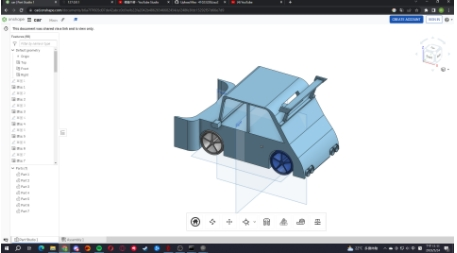
\includegraphics[width=3.75in]{41023230robot1}
\end{figure}
41023231機器人\\
\begin{figure}
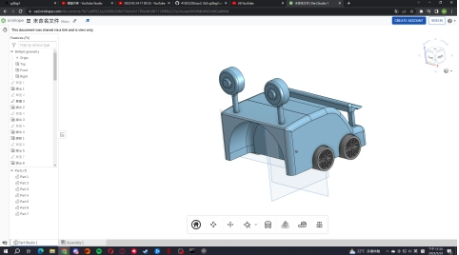
\includegraphics[width=3.75in]{41023231robot1}
\end{figure}
41023232機器人\\
\begin{figure}
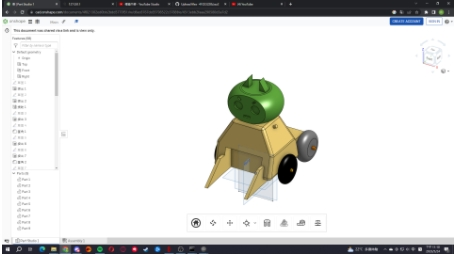
\includegraphics[width=3.75in]{41023232robot1}
\end{figure}
41023233機器人\\
\begin{figure}
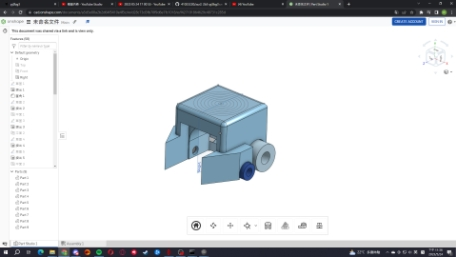
\includegraphics[width=3.75in]{41023233robot1}
\end{figure}
41023253機器人\\
\begin{figure}
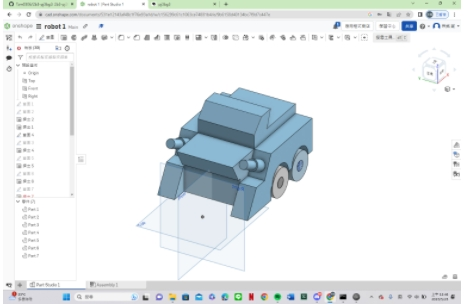
\includegraphics[width=3.75in]{41023253robot1}
\end{figure}
\section{image\_Quadricycle Second Edition}
41023233機器人\\
\begin{figure}
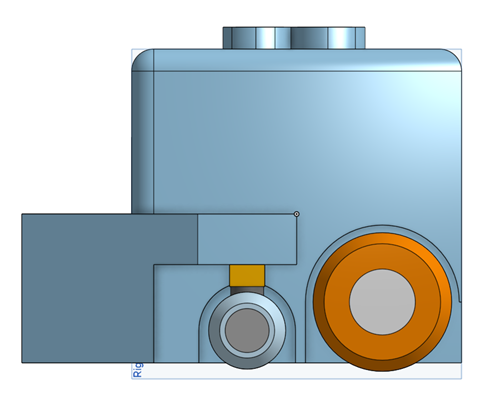
\includegraphics[width=3.75in]{41023233robot2}
\end{figure}
41023250機器人\\
\begin{figure}
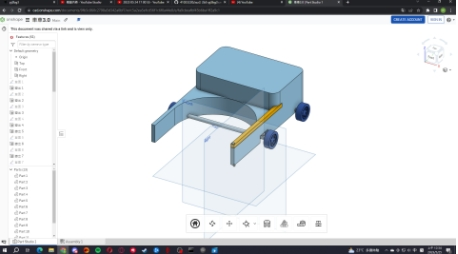
\includegraphics[width=3.75in]{41023250robot2}
\end{figure}
\section{image\_court}
球場本體\\
\begin{figure}
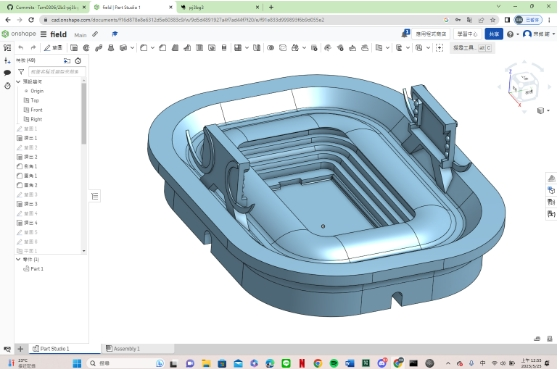
\includegraphics[width=3.75in]{court}
\end{figure}
球門\\
\begin{figure}
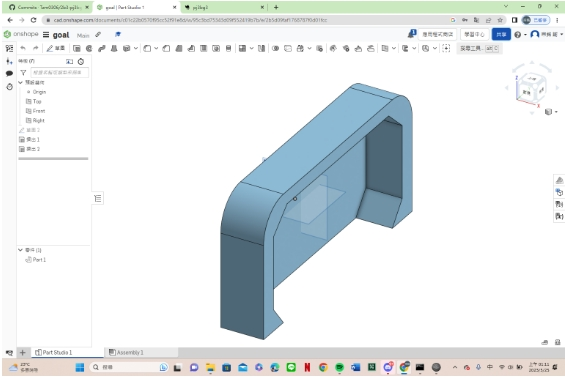
\includegraphics[width=3.75in]{goal}
\end{figure}
球場球門組合\\
\begin{figure}
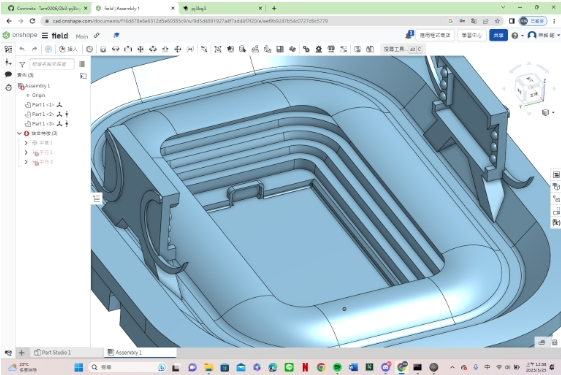
\includegraphics[width=3.75in]{court+goal}
\end{figure}
組合並加入車子\\
\begin{figure}
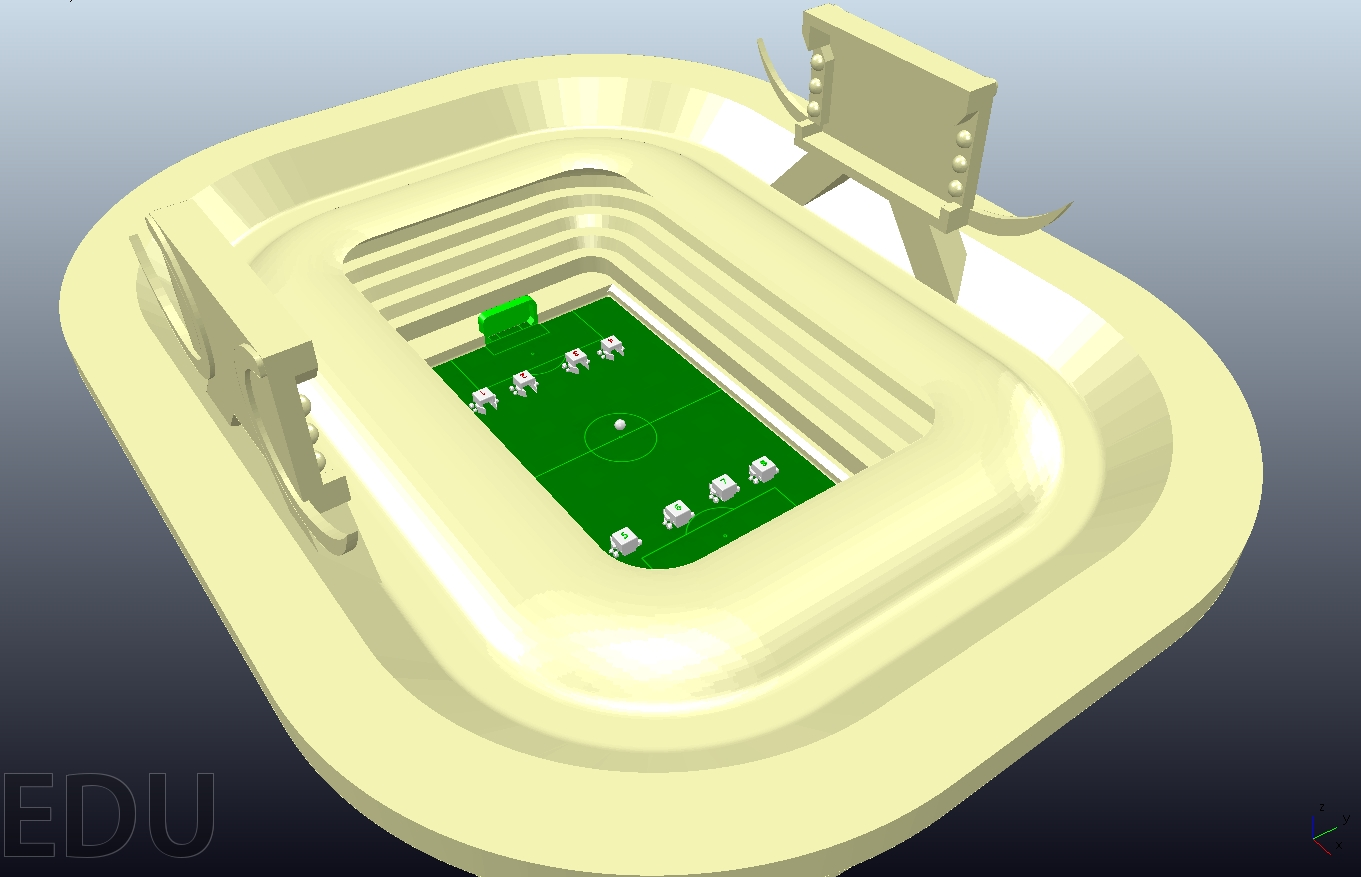
\includegraphics[width=3.75in]{race}
\end{figure}
可修改方向:將球場獨立出來,如此可把觀眾席設為non-respondable,使其模擬時速度增加。\\
經修改後的獨立球場\\
\begin{figure}
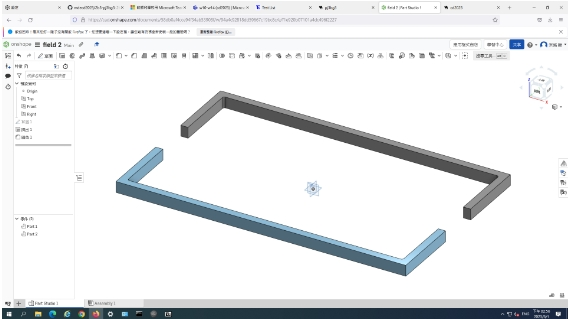
\includegraphics[width=3.75in]{Independence Stadium}
\end{figure}
\section{image\_race}
\begin{figure}
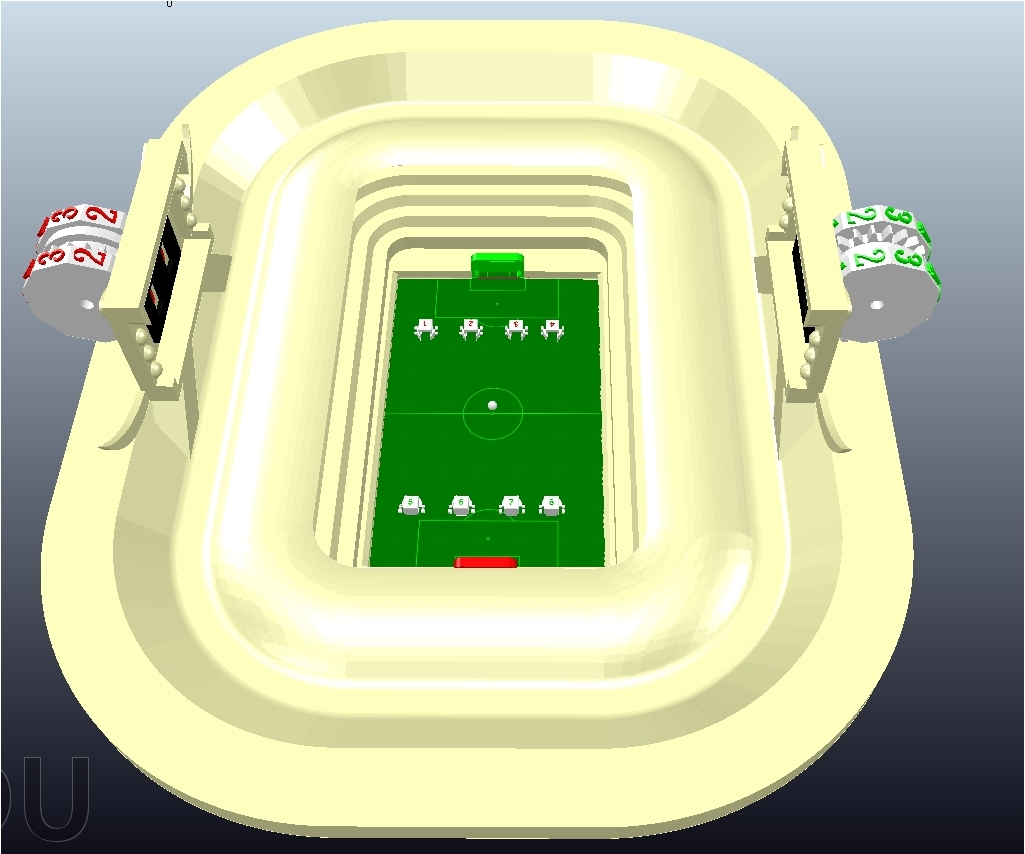
\includegraphics[width=5in]{race2}
\end{figure}




%=---------------------參考文獻----------------------=%

%=---------------附錄-----------------=%
\addcontentsline{toc}{chapter}{附錄} %新增目錄名稱

\newpage
%=-------------作者簡介-----------------=%
    \addcontentsline{toc}{chapter}{作者簡介}
    \begin{center}
	\fontsize{20pt}{0em}\selectfont \bf{作者簡介}\\
	\end{center}	
	{\begin{textblock}{6}(0,0.5)
	\begin{figure}
	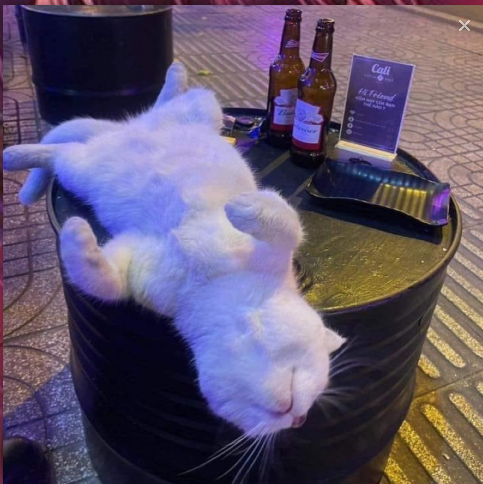
\includegraphics[width=1.25in]{41023220}  %作者照片
	\end{figure}
	\end{textblock}}
	{\renewcommand\baselinestretch{0.99}\selectfont %設定以下行距
	{\begin{textblock}{15}(3.5,0.7)%{寬度}(以左上角為原點之右移量,下移量)
	\noindent\fontsize{14pt}{0em}\selectfont \makebox[4em][s]{姓名}\enspace:\enspace
    \fontsize{14pt}{0em}\selectfont \makebox[4em][s]{陳冠珉}\\     \hspace*{\fill} \\
    \fontsize{14pt}{0em}\selectfont \makebox[4em][s]{學號}\enspace:\enspace
    \fontsize{14pt}{0em}\selectfont \makebox[4em][s]{41023220} \\ %\makebox為文本盒子
    \hspace*{\fill} \\
    \fontsize{14pt}{0em}\selectfont \makebox[4em][s]{就讀學校}\enspace:\enspace
    \fontsize{14pt}{0em}\selectfont \makebox[9em][s]{國立虎尾科技大學}\\
    \fontsize{14pt}{0em}\selectfont \makebox[5em][s]{\quad}\enspace\enspace
    \fontsize{14pt}{0em}\selectfont \makebox[8em][s]{機械設計工程系}\\
    \hspace*{\fill} \\
    \fontsize{14pt}{0em}\selectfont \makebox[4em][s]{經歷}\enspace:\enspace
    \end{textblock}}}
   % \hspace*{\fill} \\
   \vspace{2em}
	{\begin{textblock}{6}(0,2.3)
	\begin{figure}
	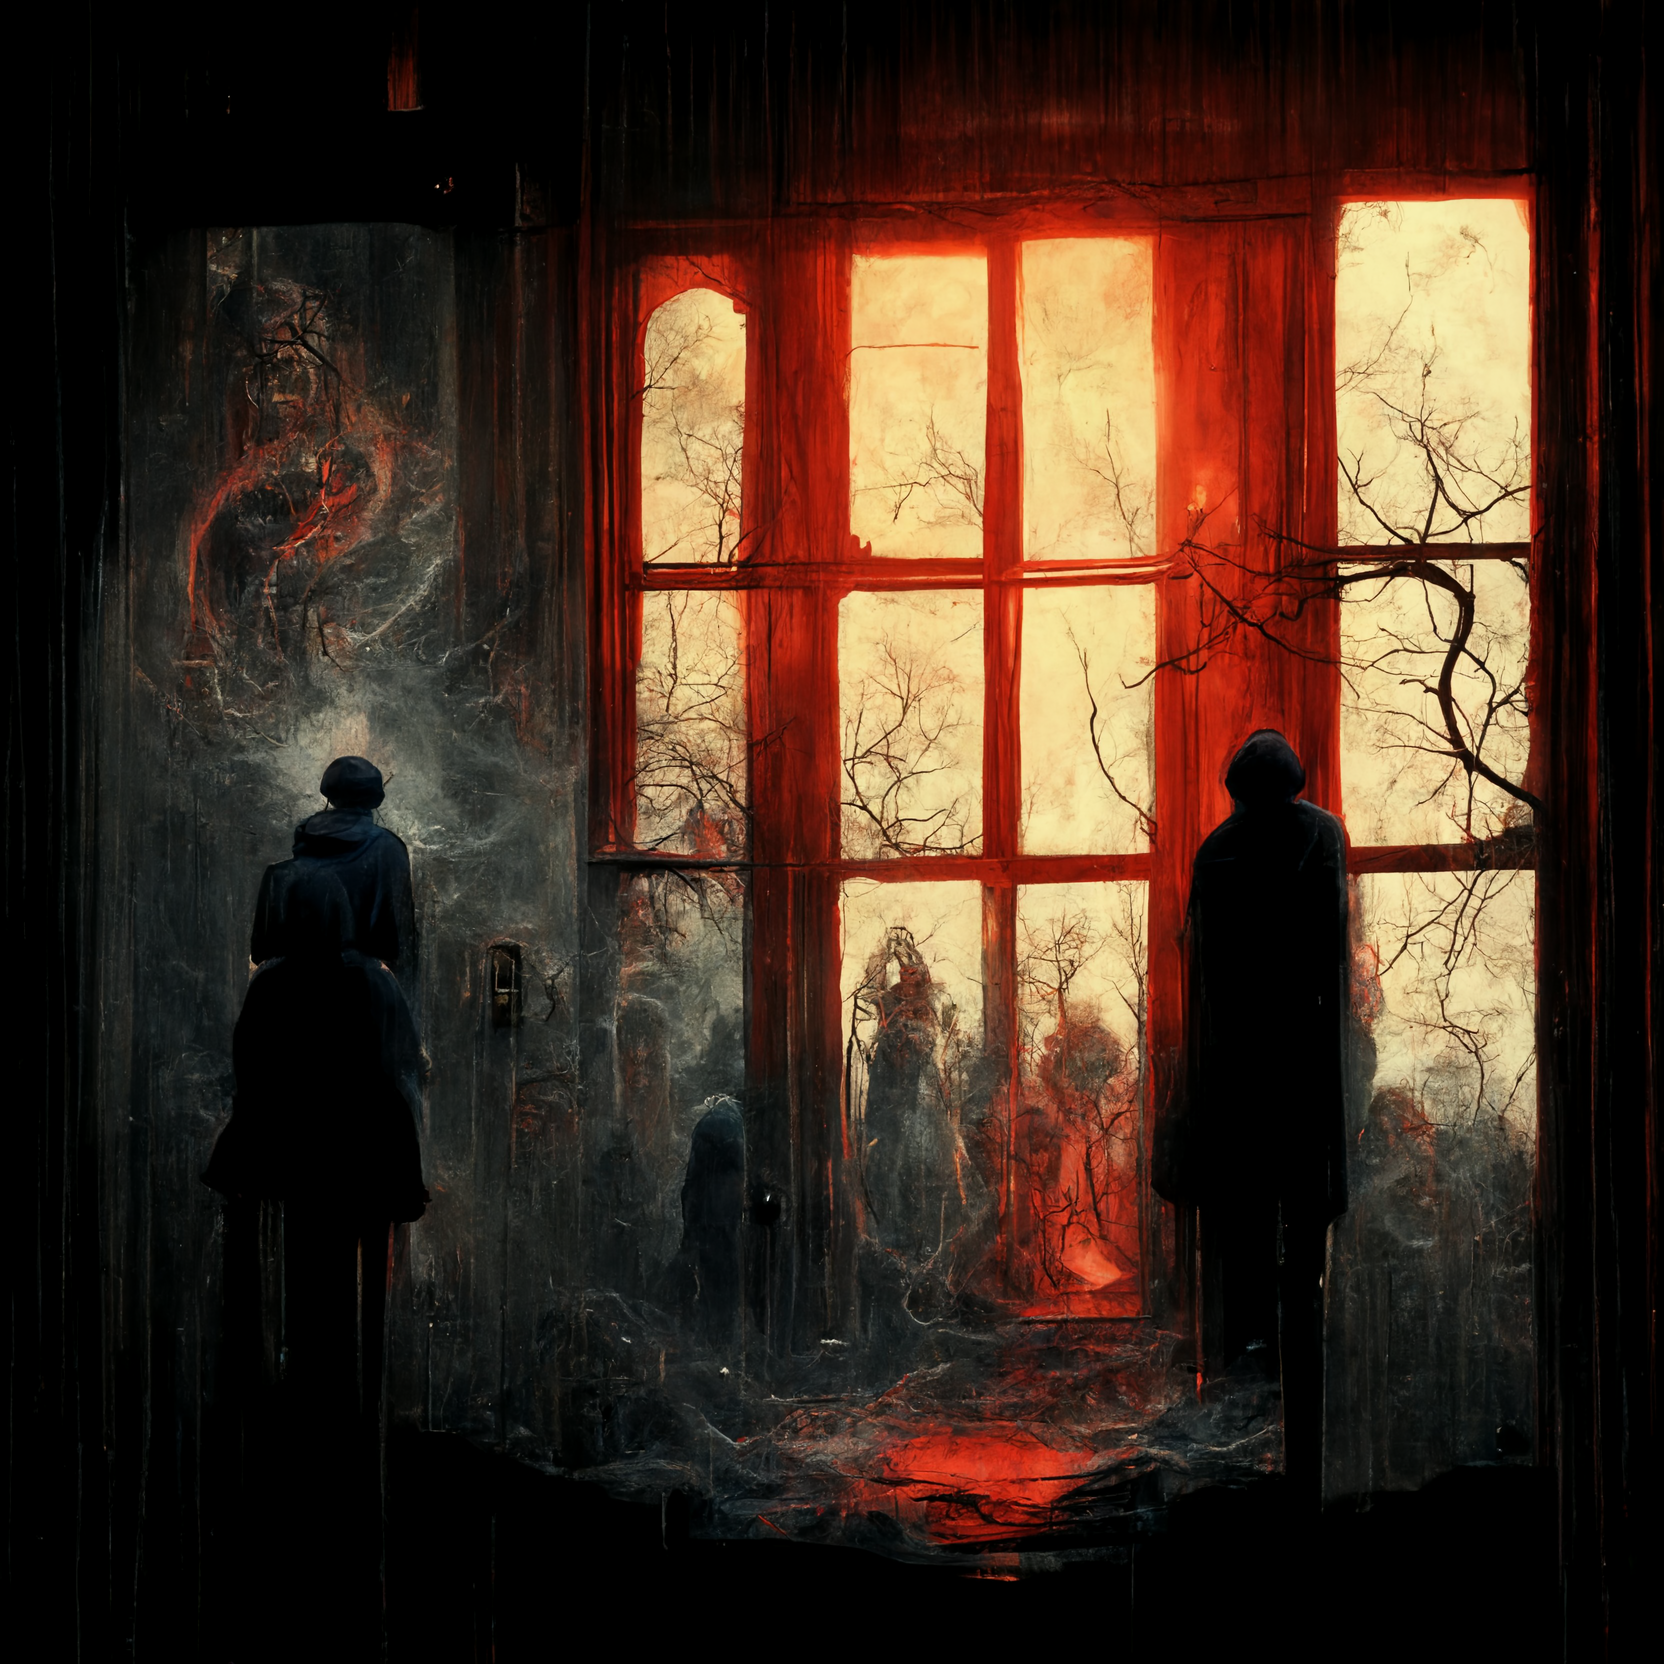
\includegraphics[width=1.15in]{41023226}  %作者照片
    \end{figure}
    \end{textblock}}
    {\renewcommand\baselinestretch{0.99}
    \selectfont %設定以下行距
    {\begin{textblock}{15}(3.5,2.5) %{寬度}(以左上角為原點之右移量,下移量)
\noindent\fontsize{14pt}{0em}\selectfont \makebox[4em][s]{姓名}\enspace:\enspace
\fontsize{14pt}{0em}\selectfont \makebox[4em][s]{陳建霖}\\ 
\hspace*{\fill} \\
\fontsize{14pt}{0em}\selectfont \makebox[4em][s]{學號}\enspace:\enspace
\noindent\fontsize{14pt}{0em}\selectfont \makebox[4em][s]{41023226} \\ 
\hspace*{\fill} \\
\fontsize{14pt}{0em}\selectfont \makebox[4em][s]{就讀學校}\enspace:\enspace
\fontsize{14pt}{0em}\selectfont \makebox[9em][s]{國立虎尾科技大學}\\
\fontsize{14pt}{0em}\selectfont \makebox[5em][s]{\quad}\enspace\enspace
\fontsize{14pt}{0em}\selectfont \makebox[8em][s]{機械設計工程系}\\
\hspace*{\fill} \\
\fontsize{14pt}{0em}\selectfont \makebox[4em][s]{經歷}\enspace:\enspace
    \end{textblock}}}
   % \hspace*{\fill} \\
   \vspace{2em}
	{\begin{textblock}{6}(0,4.1)
	\begin{figure}
	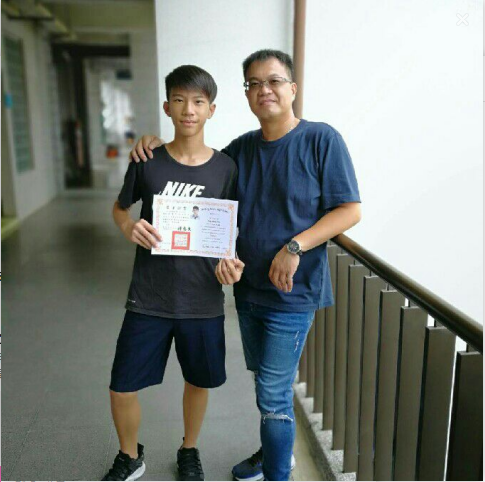
\includegraphics[width=1.15in]{41023230}  %作者照片
    \end{figure}
    \end{textblock}}
    {\renewcommand\baselinestretch{0.99}
    \selectfont %設定以下行距
    {\begin{textblock}{15}(3.5,4.3) %{寬度}(以左上角為原點之右移量,下移量)
\noindent\fontsize{14pt}{0em}\selectfont \makebox[4em][s]{姓名}\enspace:\enspace
\fontsize{14pt}{0em}\selectfont \makebox[4em][s]{彭聖宗}\\ 
\hspace*{\fill} \\
\fontsize{14pt}{0em}\selectfont \makebox[4em][s]{學號}\enspace:\enspace
\noindent\fontsize{14pt}{0em}\selectfont \makebox[4em][s]{41023230} \\ 
\hspace*{\fill} \\
\fontsize{14pt}{0em}\selectfont \makebox[4em][s]{就讀學校}\enspace:\enspace
\fontsize{14pt}{0em}\selectfont \makebox[9em][s]{國立虎尾科技大學}\\
\fontsize{14pt}{0em}\selectfont \makebox[5em][s]{\quad}\enspace\enspace
\fontsize{14pt}{0em}\selectfont \makebox[8em][s]{機械設計工程系}\\
\hspace*{\fill} \\
\fontsize{14pt}{0em}\selectfont \makebox[4em][s]{經歷}\enspace:\enspace
    \end{textblock}}}
   % \hspace*{\fill} \\
   \vspace{2em}
	{\begin{textblock}{6}(0,5.9)
	\begin{figure}
	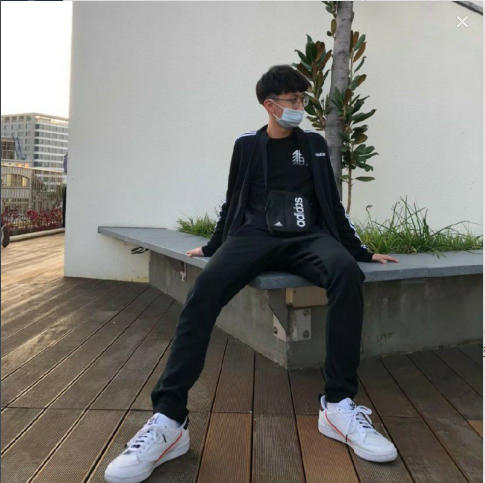
\includegraphics[width=1.15in]{41023231}  %作者照片
    \end{figure}
    \end{textblock}}
    {\renewcommand\baselinestretch{0.99}
    \selectfont %設定以下行距
    {\begin{textblock}{15}(3.5,6.1) %{寬度}(以左上角為原點之右移量,下移量)
\noindent\fontsize{14pt}{0em}\selectfont \makebox[4em][s]{姓名}\enspace:\enspace
\fontsize{14pt}{0em}\selectfont \makebox[4em][s]{湛有杰}\\ 
\hspace*{\fill} \\
\fontsize{14pt}{0em}\selectfont \makebox[4em][s]{學號}\enspace:\enspace
\noindent\fontsize{14pt}{0em}\selectfont \makebox[4em][s]{41023231} \\ 
\hspace*{\fill} \\
\fontsize{14pt}{0em}\selectfont \makebox[4em][s]{就讀學校}\enspace:\enspace
\fontsize{14pt}{0em}\selectfont \makebox[9em][s]{國立虎尾科技大學}\\
\fontsize{14pt}{0em}\selectfont \makebox[5em][s]{\quad}\enspace\enspace
\fontsize{14pt}{0em}\selectfont \makebox[8em][s]{機械設計工程系}\\
\hspace*{\fill} \\
\fontsize{14pt}{0em}\selectfont \makebox[4em][s]{經歷}\enspace:\enspace
    \end{textblock}}}
   % \hspace*{\fill} \\
   \vspace{2em}
	{\begin{textblock}{6}(0,7.7)
	\begin{figure}
	
\includegraphics[width=1.15in]{41023232}  %作者照片
    \end{figure}
    \end{textblock}}
    {\renewcommand\baselinestretch{0.99}
    \selectfont %設定以下行距
    {\begin{textblock}{15}(3.5,7.9) %{寬度}(以左上角為原點之右移量,下移量)
\noindent\fontsize{14pt}{0em}\selectfont \makebox[4em][s]{姓名}\enspace:\enspace
\fontsize{14pt}{0em}\selectfont \makebox[4em][s]{雲敬家}\\ 
\hspace*{\fill} \\
\fontsize{14pt}{0em}\selectfont \makebox[4em][s]{學號}\enspace:\enspace
\noindent\fontsize{14pt}{0em}\selectfont \makebox[4em][s]{41023233} \\ 
\hspace*{\fill} \\
\fontsize{14pt}{0em}\selectfont \makebox[4em][s]{就讀學校}\enspace:\enspace
\fontsize{14pt}{0em}\selectfont \makebox[9em][s]{國立虎尾科技大學}\\
\fontsize{14pt}{0em}\selectfont \makebox[5em][s]{\quad}\enspace\enspace
\fontsize{14pt}{0em}\selectfont \makebox[8em][s]{機械設計工程系}\\
\hspace*{\fill} \\
\fontsize{14pt}{0em}\selectfont \makebox[4em][s]{經歷}\enspace:\enspace
    \end{textblock}}}
    %\hspace*{\fill} \\

\newpage
%=-------------作者簡介2-----------------=%
    \addcontentsline{toc}{chapter}{作者簡介2}
    \begin{center}
	\fontsize{20pt}{0em}\selectfont \bf{作者簡介2}\\
	\end{center}	
    %\hspace*{\fill} \\
    \vspace{2em}
    {\begin{textblock}{6}(0,0.5)
    \begin{figure}
        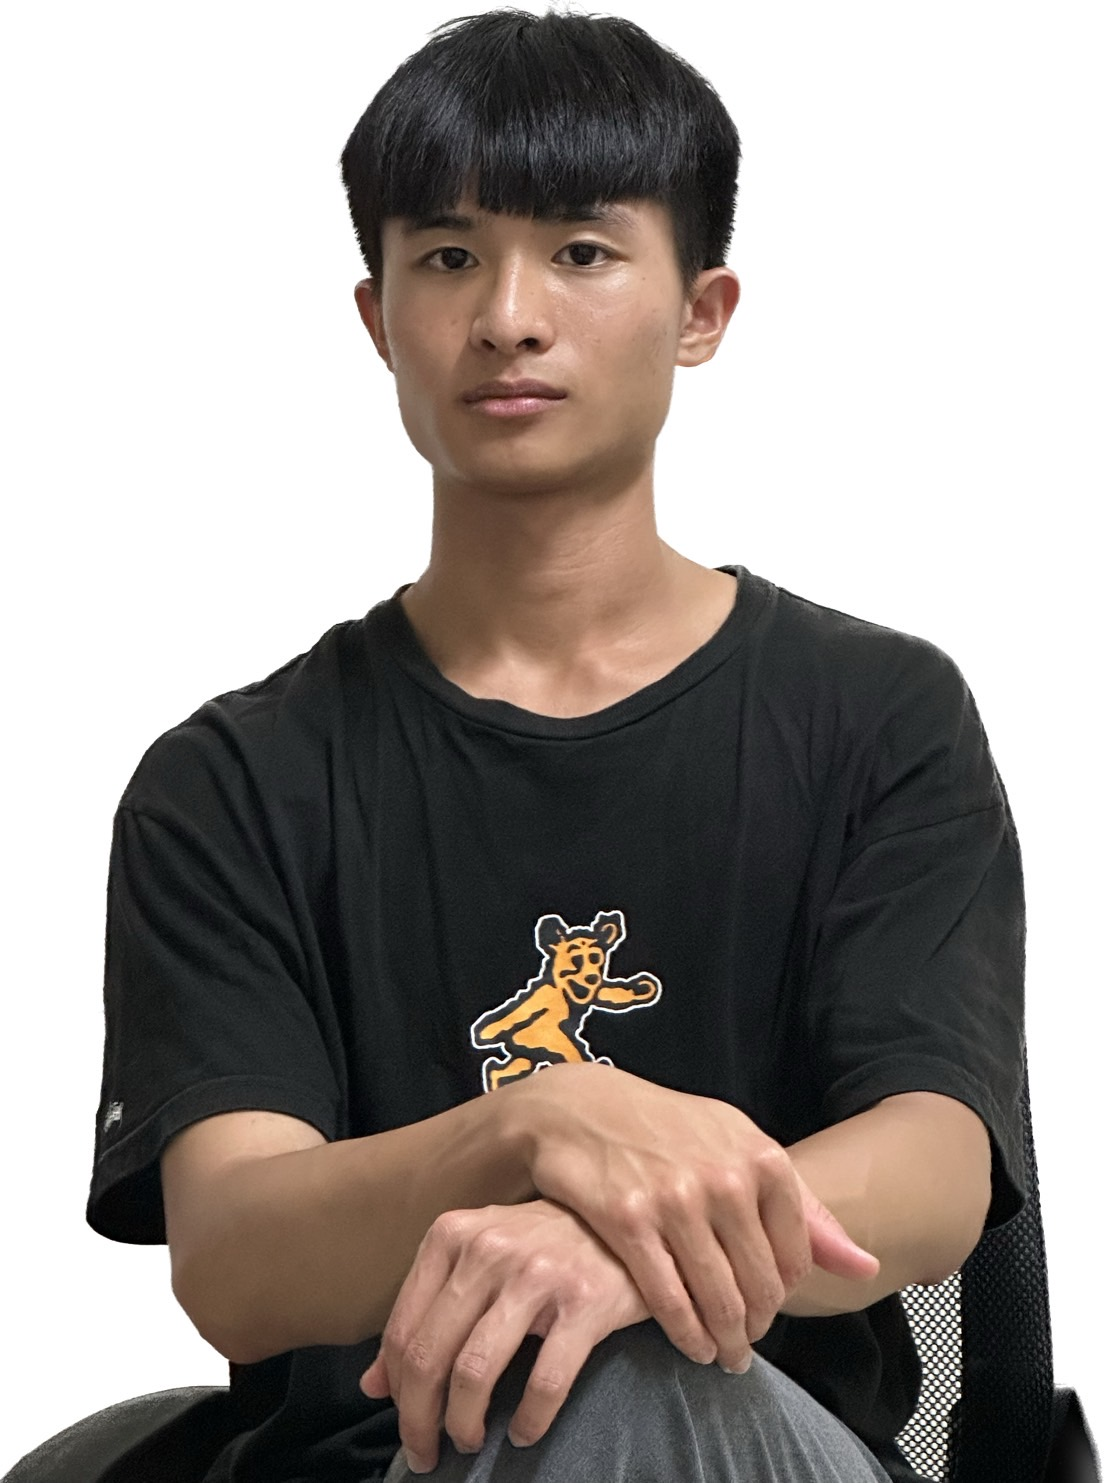
\includegraphics[width=1.15in]{41023233} %{}內是圖片文件的相對路徑
    \end{figure}
    \end{textblock}}
    {\renewcommand\baselinestretch{0.99}\selectfont %設定以下行距
    {\begin{textblock}{15}(3.5,0.7) %{寬度}(以左上角為原點之右移量,下移量)
\noindent\fontsize{14pt}{0em}\selectfont \makebox[4em][s]{姓名}\enspace:\enspace%\noindent指定首行不進行縮排
\fontsize{14pt}{0em}\selectfont \makebox[4em][s]{黃文彥}\\ 
\hspace*{\fill} \\
\noindent\fontsize{14pt}{0em}\selectfont \makebox[4em][s]{學號}\enspace:\enspace
\noindent\fontsize{14pt}{0em}\selectfont \makebox[4em][s]{41023233} \\ %\makebox為文本盒子
\hspace*{\fill} \\
\noindent\fontsize{14pt}{0em}\selectfont \makebox[4em][s]{就讀學校}\enspace:\enspace
\noindent\fontsize{14pt}{0em}\selectfont \makebox[9em][s]{國立虎尾科技大學}\\
\noindent\fontsize{14pt}{0em}\selectfont \makebox[5em][s]{\quad}\enspace\enspace
\noindent\fontsize{14pt}{0em}\selectfont \makebox[8em][s]{機械設計工程系}\\
\hspace*{\fill} \\
\noindent\fontsize{14pt}{0em}\selectfont \makebox[4em][s]{經歷}\enspace:\enspace
    \end{textblock}}}
   % \hspace*{\fill} \\
   \vspace{2em}
	{\begin{textblock}{6}(0,2.3)
	\begin{figure}
	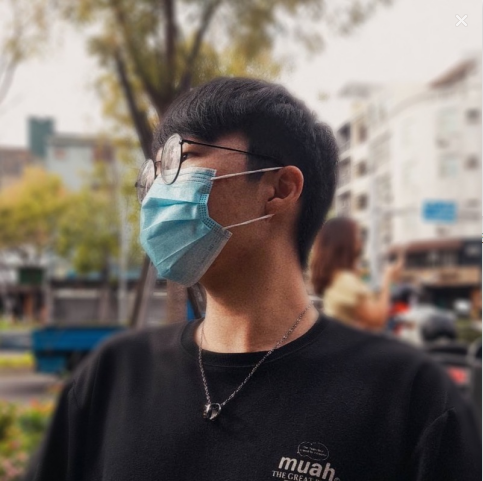
\includegraphics[width=1.15in]{41023250}  %作者照片
    \end{figure}
    \end{textblock}}
    {\renewcommand\baselinestretch{0.99}
    \selectfont %設定以下行距
    {\begin{textblock}{15}(3.5,2.5) %{寬度}(以左上角為原點之右移量,下移量)
\noindent\fontsize{14pt}{0em}\selectfont \makebox[4em][s]{姓名}\enspace:\enspace
\fontsize{14pt}{0em}\selectfont \makebox[4em][s]{蔡叡得}\\ 
\hspace*{\fill} \\
\fontsize{14pt}{0em}\selectfont \makebox[4em][s]{學號}\enspace:\enspace
\noindent\fontsize{14pt}{0em}\selectfont \makebox[4em][s]{41023250} \\ 
\hspace*{\fill} \\
\fontsize{14pt}{0em}\selectfont \makebox[4em][s]{就讀學校}\enspace:\enspace
\fontsize{14pt}{0em}\selectfont \makebox[9em][s]{國立虎尾科技大學}\\
\fontsize{14pt}{0em}\selectfont \makebox[5em][s]{\quad}\enspace\enspace
\fontsize{14pt}{0em}\selectfont \makebox[8em][s]{機械設計工程系}\\
\hspace*{\fill} \\
\fontsize{14pt}{0em}\selectfont \makebox[4em][s]{經歷}\enspace:\enspace
    \end{textblock}}}
   % \hspace*{\fill} \\
   \vspace{2em}
    {\begin{textblock}{6}(0,4.1)
    \begin{figure}
        
\includegraphics[width=1.15in]{41023253} %{}內是圖片文件的相對路徑
    \end{figure}
    \end{textblock}}
    {\renewcommand\baselinestretch{0.99}\selectfont %設定以下行距
    {\begin{textblock}{15}(3.5,4.3) %{寬度}(以左上角為原點之右移量,下移量)
\noindent\noindent\fontsize{14pt}{0em}\selectfont \makebox[4em][s]{姓名}\enspace:\enspace
\noindent\fontsize{14pt}{0em}\selectfont \makebox[4em][s]{謝宗銘}\\ \hspace*{\fill} \\
\noindent\fontsize{14pt}{0em}\selectfont \makebox[4em][s]{學號}\enspace:\enspace
\noindent\fontsize{14pt}{0em}\selectfont \makebox[4em][s]{41023253} \\ \hspace*{\fill} \\
\noindent\fontsize{14pt}{0em}\selectfont \makebox[4em][s]{就讀學校}\enspace:\enspace
\noindent\fontsize{14pt}{0em}\selectfont \makebox[9em][s]{國立虎尾科技大學}\\
\noindent\fontsize{14pt}{0em}\selectfont \makebox[5em][s]{\quad}\enspace\enspace
\noindent\fontsize{14pt}{0em}\selectfont \makebox[8em][s]{機械設計工程系}\\
\hspace*{\fill} \\
\noindent\fontsize{14pt}{0em}\selectfont \makebox[4em][s]{經歷}\enspace:\enspace
    \end{textblock}}}
    %\hspace*{\fill} \\

\newpage
%=----------------書背----------------------=%
\pagestyle{empty}%設定沒有頁眉和頁腳
\begin{center}
\fontsize{0.001pt}{1pt}\selectfont .\\
\vspace{4em}
\fontsize{30pt}{30pt}\selectfont 【13】 \\
\fontsize{20pt}{20pt}\selectfont
\vspace{0.5em}
分\\
類\\
編\\
號\\
\vspace{0.5em}
\hspace{-0.5em}:\\
\vspace{0.5em}
\rotatebox[origin=cc]{270}{\sectionef\LARGE \textbf{pj3bg3}}\\ %旋轉
\vspace{0.5em}
網\\
際\\
足\\
球\\
場\\
景\\
設\\
計\\
\vspace{2em}
一\\
一\\
二\\
級\\

\end{center}
%\newpage
%\begin{landscape}  %橫式環境
%\begin{center}
%\fontsize{0.001pt}{1pt}\selectfont .
%\vspace{70mm}
%\rotatebox[origin=cc]{90}{\LARGE 【14】}\rotatebox[origin=cc]%{180}{\LARGE 1-2-APP-8765} %旋轉
%\end{center}
%\end{landscape}
\end{document}
